\begin{figure}[htb]
    \begin{center}
    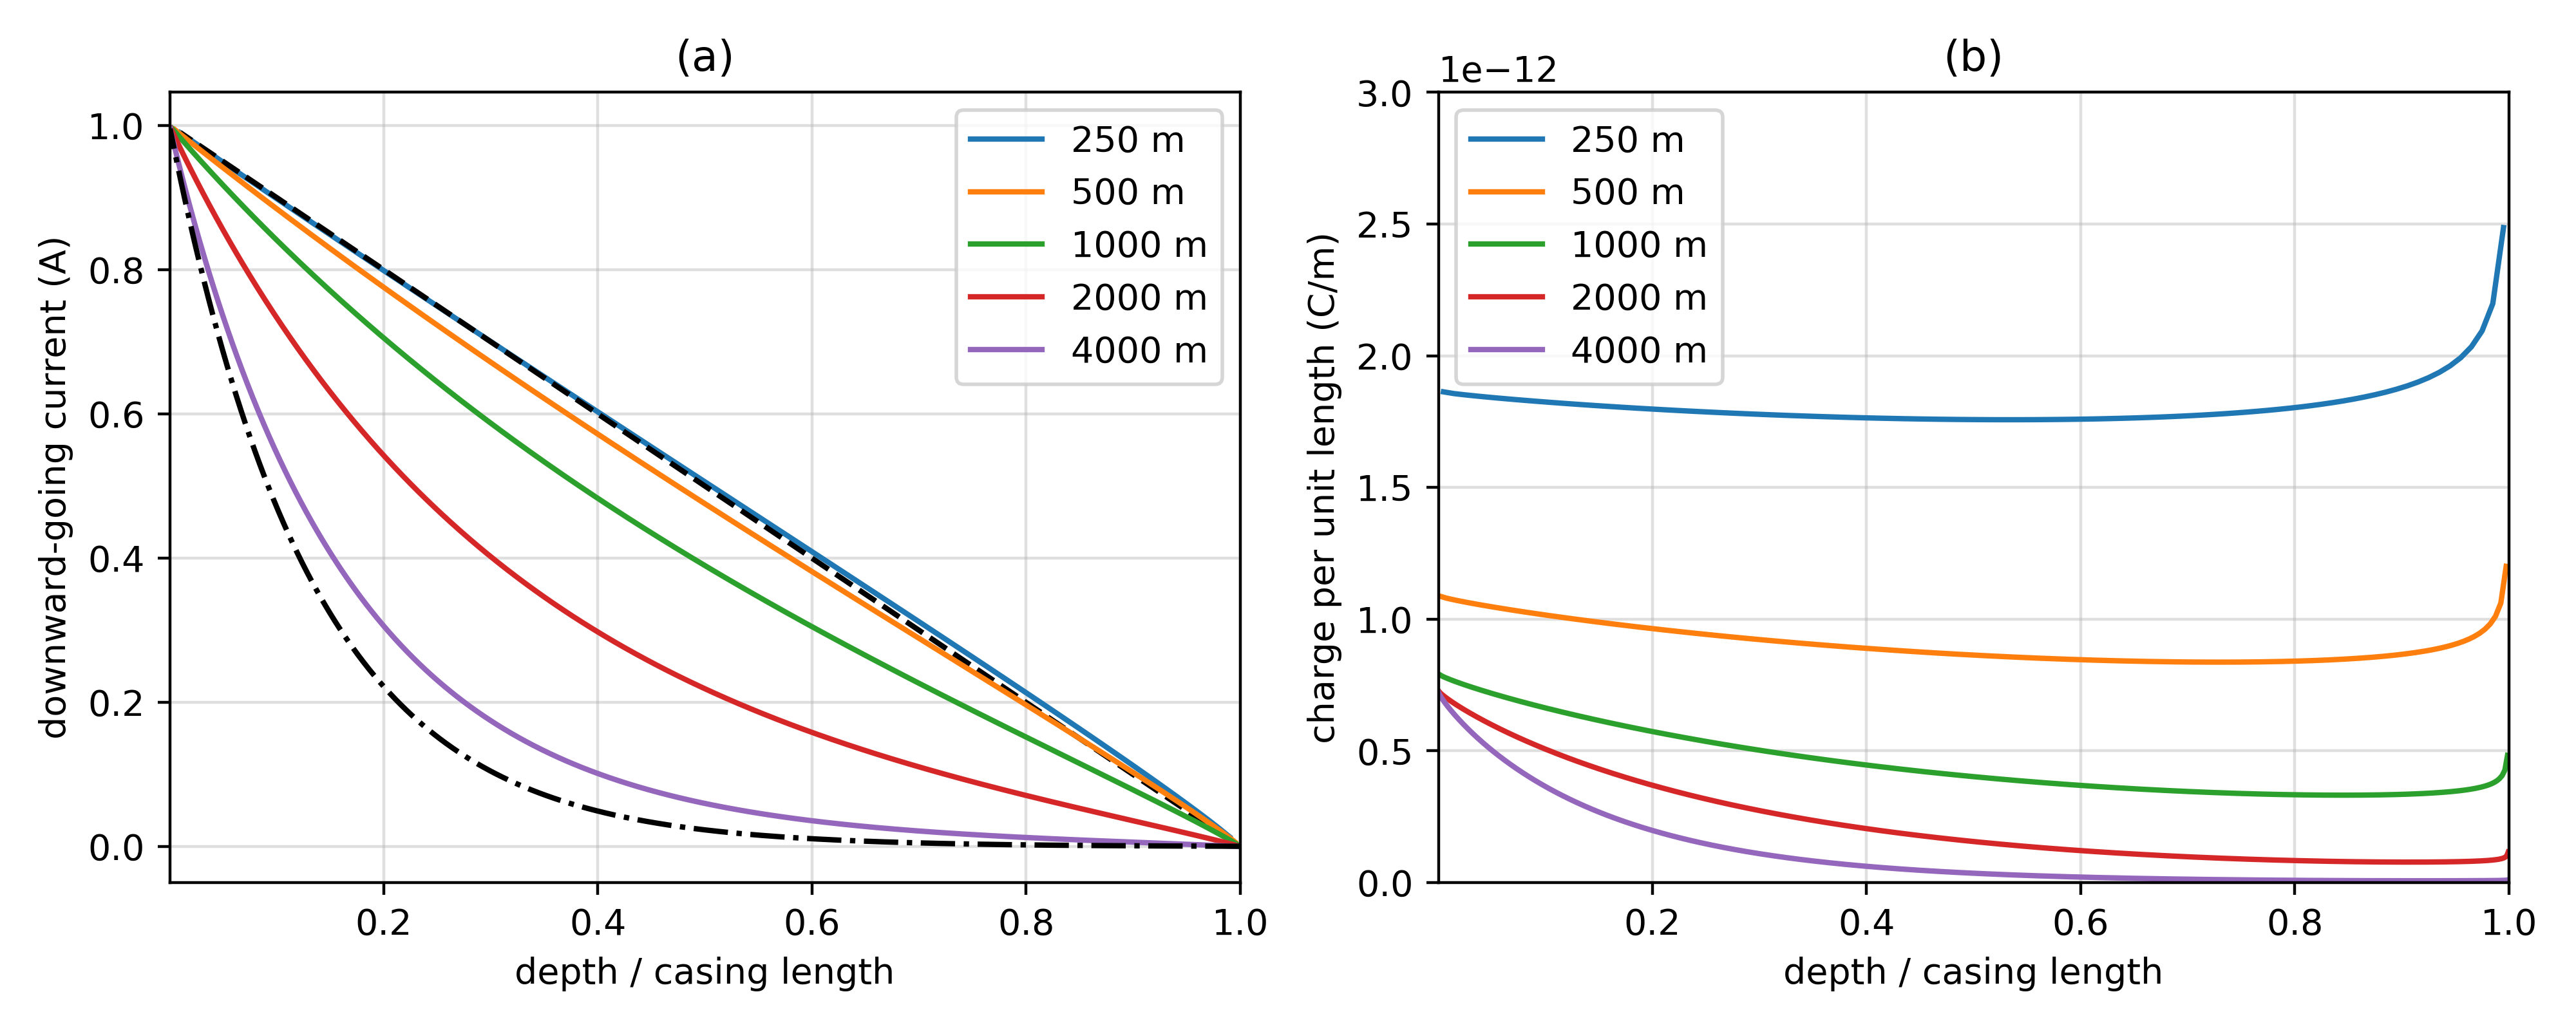
\includegraphics[width=\columnwidth]{figures/kaufman_finite_well.png}
    \end{center}
\caption{
    (a) Current along a well for 5 different wellbore lengths.
    The x-axis is depth normalized by the length of the well. The black
    dashed line shows the short-well approximation (equation 45 in \cite{Kaufman1993})
    for a 200m long well. The black dash-dot line shows the long-well approximation
    (equation 53 in \cite{Kaufman1993}) for a 4000m well.
    (b) Charge per unit length along the well for 5 different wellbore lengths.
}
\label{fig:kaufman_finite_well}
\end{figure}
